%\documentclass[a4paper,10pt]{article}
%\usepackage[utf8]{inputenc}
%\usepackage{graphicx}
%\usepackage{url}

%opening
%\title{Evacuation Simulator}
%\author{Team L}

%\begin{document}

%\maketitle

%\begin{abstract}
%It is acknowledged that the cost of 
%running evacuation drills in public environments is relatively high both in time and money. This is because very often, the 
%evacuation drills have to be run at night where the chosen environment is not in service and consequently additional payments for 
%equipments, hiring evacuees and fire consultant are needed. This results in fewer number of evacuation drills. 
%There are also some types of evacuation that cannot be drilled both safely and accurately such as a large fire.
%An evacuation simulator is a possible solution to these problems which uses human behaviour in evacuation environment 
%to predict the egress of a population. The aim of this project involves producing a three dimensions visualised 
%evacuation simulator at The Tall Ship at Riverside, Glasgow. Not only focussing on implementation side, the research 
%side is essentially indispensable. Psychology of mass emergency evacuation behaviour and crowd patterns are applied in 
%order to best determine how people will react in an evacuation situation. Moreover, several path finding algorithms 
%are studied to find out which one is suitable for the project.
%The implementation side of this project 
%involves the modelling of the chosen environment in 3D visualisation and simulating an evacuation on this model.
%With this combination, evacuation simulator is more realistic.
%\end{abstract}
%
%\tableofcontents

\section{Introduction}

\subsection{Definition of an Evacuation Simulator}
An evacuation simulator can be defined as a system to determine evacuation
times by predicting the egress of individuals in a building or similar
structure~\cite{evacuationSimulatordefinition}. They are used for the identification of weaknesses in the design of buildings which could detrimentally affect the egress of persons in an evacuation and to aid personnel in preparing for an evacuation~\cite{evacuationModel}.

\subsection{Why Implement an Evacuation Simulator}
The task of testing a building's evacuation procedure can be
both difficult and expensive. One approach is to hire members of the public
as stand-in ``evacuees'' and run a mock evacuation, such as those performed as part of Forward Defensive
in preparation for the London 2012 Olympics \cite{DailyMailEvacuation}. In theory, this would allow an 
appropriate expert such as a consultant from a local fire department to assess the effectiveness
of an existing plan. However, such tests on public buildings can be very expensive: the cost
of hiring evacuees could be significant. Also certain aspects of evacuations, such
as testing the possibility of a crush, can expose participants
to real danger. Finally if an evacuee knows they are participating in an experiment
their behaviour is inherently different than it would be in a real evacuation. This
phenomenon is known as Evaluation Apprehension\cite{EvalApprehension}.\\
For these reasons large scale tests on a building are rarely performed.
What a simulator provides is a means for an expert to extensively test the outcomes of evacuating a location
at minimal cost. By configuring variables in the simulation the expert can examine the probable outcome of multiple evacuations
and look for potential sources of danger in a building or evacuation procedure.\\

Of particular note is the ability to investigate the effects of human behaviour on the success of an evacuation. This ability is central to a successful system and it is desirable to model the behaviour of the population as accurately as is achievable \cite{psychology}.


\subsection{Aims}
The project's aims are driven by the desire to maximise the flexibility and extensibility of the system, and to make the system as accurate as is achievable within the time available. The four key aims can be summarised as follows.

\subsubsection{A Multi-Agent Model of Individuals and Individual Behaviour}
Previous projects have emphasised crowd behaviour: they have modelled the population from a top down 
perspective with little consideration for the perception and interaction which an individual experiences in an evacuation.
One of the primary aims of this project is to represent an accurate model of individual behaviour.
Previous work has shown that multi-agent systems can achieve this. By taking this approach ``the full effects of diversity that exists among agents in their attributes and behaviours can be observed as it
gives rises to the behaviour of the system as a whole'' \cite{AgentBasedTutorial}.

\subsubsection{Use of up-to-date technologies wherever possible}
Even in recently developed simulators, now deprecated technologies such as Java3D are being used. This limits their future extensibility greatly and is not desirable.
The underlying technologies used in development were chosen primarily based on their future potential and strength of community support.
These are discussed extensively in the Research chapter.

\subsubsection{Use of Navigation Meshes in Environment Modelling}
A Navigation Mesh is a graph representation of an environment in terms of a set of convex polygons which describe the `walk able' surface of an environment. This design aids agents in finding paths through large areas, whilst avoiding static obstacles in the environment.
This technique has largely been pioneered in gaming, but is equally applicable in this setting. The benefits of a navigation mesh, or `navmesh' is that it allows agents to move 
freely compared to other techniques such as representing the environment using a grid. A navmesh is typically combined with the powerful path finding algorithm A* to 
optimise agent movement \cite{A*Review}.

\subsection{Prerequisites}
Where possible all technical concepts used within this paper will be clearly defined. However, to fully understand the remainder of this report, the reader should have at least
some knowledge of the following concepts:
\begin{itemize}
 \item Object-Oriented programming concepts (preferably in Java)
 \item Concurrent programming concepts
 \item Pathfinding simulation and collision detection/avoidance~\cite{gameProgramming}~\cite{collisionDetection}
 \item Herding, flocking behaviour and boids~\cite{HAndBoid}~\cite{Fbehavior}
 \item Human behavioural traits~\cite{HumanBehaviouralTraits}
\end{itemize}

\subsection{Previous Work}

\subsubsection{Fluid Based Systems}
These systems model crowd movement as if the crowd were a fluid \cite{WikipediaFluidMechanics}, using equations and principles taken from Physics. 
Exodus \cite{GaleaNumericalSimulation,GaleaMathModelling} is an example of such a system. There are drawbacks in such a style 
of simulator. Crowds ``have a choice in their direction, they have no conservation of momentum and can stop and start at will" \cite{StillCrowdDynamics}. 
These concepts are not accounted for in fluid models, and so this style of simulator is limited to estimating the movement of a crowd as a whole without
considering individual interactions.

\subsubsection{Matrix or Grid Based Systems}
In a matrix or grid based system, the floor of the environment is represented by a series of adjacent nodes, often square or hexagonal in shape. Each 
cell can represent open areas, areas blocked by a static obstacle, exits, etc. This method is becoming less common, but two formerly well-known examples are 
Egress and Pedroute. It was suggested that the existing matrix-based models suffer from the
difficulties of simulating crowd cross flow and concourses. Furthermore, the
assumptions employed in these models are questionable when compared with field observations \cite{StillCrowdDynamics}.

\subsubsection{Emergent Agent Based Systems}
The final class of simulator we discuss here is the emergent (agent-based) simulator. In this approach the system is composed of autonomous
and interacting ``agents''. Agents interact within an environment using a defined set of simple relationships. The benefit of this approach is the introduction
of \emph{emergent} behaviour: ``patterns, structures and behaviours emerge that were not explicitly programmed into the models, but arise as the 
result of agent interactions'' \cite{AgentBasedTutorial}.\\
The MASSEgress project developed at Stanford University is an ongoing effort to develop a framework for the development of such systems \cite{MultiAgentFramework}.
It has also led to the production of at least one prototype implementing this framework. 
This project has utilised a modified version of this framework for the integration
of agent behaviour. This is discussed further in Sections \ref{Res:sec:humanBehaviour} \& \ref{Imp:sec:perceiveDecideAct}.


\section{Environment}
For the purposes of designing and evaluating the system it was necessary to choose a readily available location to be used as the 3D model with which the system operates. By choosing such a location there is the potential to run mock evaluations and other tests in the future. The environment chosen is the Tall Ship at Riverside, Glasgow \cite{TallShipSite}.

\begin{figure}
\centering
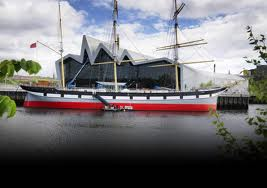
\includegraphics{../images/glasgowTallShip.jpg}
\caption{Glasgow Tall Ship}
\end{figure}

The Tall Ship was chosen as the simulation environment because:
\begin{itemize}
 \item It serves as both a tourist attraction and a function hall below decks.
 \item The ship is permanently docked and can be considered a static structure.
 \item Events can host up to 200 guests, excluding staff.
 \item It has a sufficiently complex structure in which to explore simulation techniques.
 \item No full scale evacuations have ever been held before - only staff have been used.
 \item These drills are infrequent.
\end{itemize}

\begin{figure}
\centering
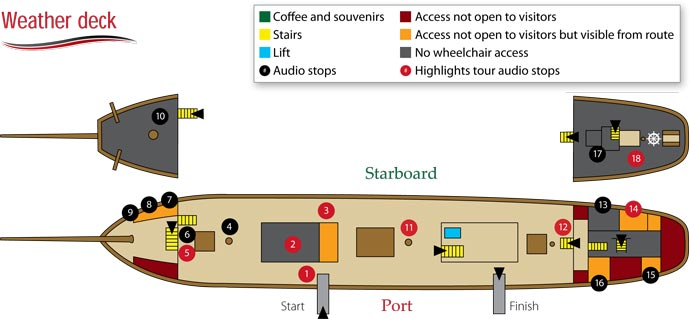
\includegraphics[scale=0.4]{../images/weatherdeck.jpg}
\caption{Weather Deck}
\end{figure}

\begin{figure}
\centering
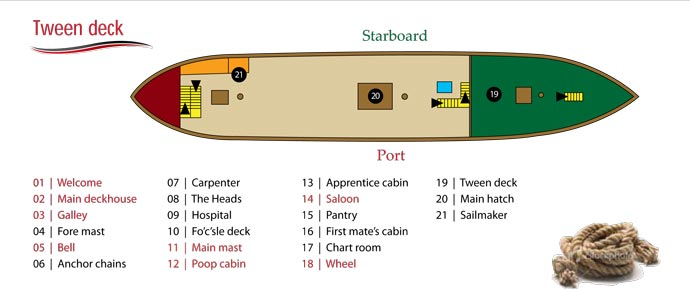
\includegraphics[scale=0.4]{../images/tweendeck.jpg}
\caption{Tween Deck}
\end{figure}

\begin{figure}
\centering
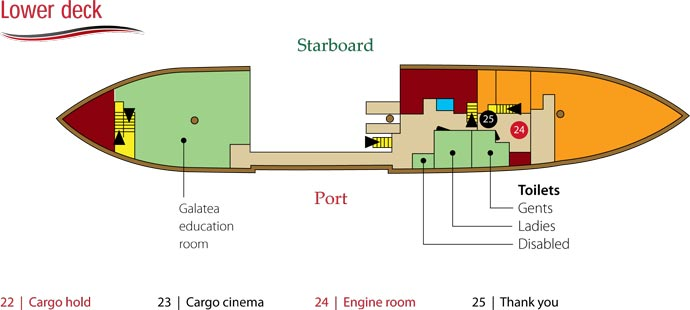
\includegraphics[scale=0.4]{../images/lowerdeck.jpg}
\caption{Lower Deck}
\end{figure}

\begin{figure}
\centering
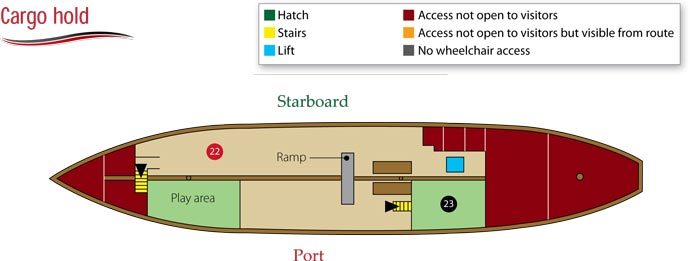
\includegraphics[scale=0.4]{../images/cargohold.jpg}
\caption{Cargo Hold}
\end{figure}

It is important to note that only small scale staff evacuations have been conducted on the ship
due to the impractical nature of carrying out an evacuation with
actual visitors. Because of this restriction, an evacuation simulation of The
Tall Ship is ideal to assess the safety of visitors on the ship in the event of an
emergency evacuation.

%\bibliographystyle{unsrt}   % this means that the order of references
%			    % is dtermined by the order in which the
%			    % \cite and \nocite commands appear
%\bibliography{individual_ref}

%\end{document}
